\section{Lista de materiales}\label{sec:materiales}

\subsection{Materiales del cartel}

\subsubsection{Componentes del módulo esclavo}
Para poder armar este módulo es necesario contar con los siguientes componentes:
\begin{itemize}
    \item 64 LEDs.
    \item Un PCB con dimesiones minimas de 7x7cm.
    \item Un MAX7219.
    \item Un capacitor polarizado 10µF.
    \item Un capacitor no polarizado 0.1µF.
    \item Una resistencia 24KOhm.
    \item Dos conector hembra 8 Pin (25.4mm): para la conexión de la matriz de LEDs.
    \item Dos conector hembra 5 Pin (25.4mm): para la interfaz entre módulos.
    \item Dos regleta de 1x12 pines hembra (1.27mm): para la conexión del MAX7219.
\end{itemize}    

\subsubsection{Componentes del módulo master}
Para poder armar este módulo es necesario contar con los siguientes componentes:
\begin{itemize}
    \item Un NodeMCU Esp8266.
    \item Un PCB con dimesiones minimas de 7x7cm.
    \item Tres transistor NPN.
    \item Seis Resistencia de 10KOmh.
    \item Cuatro Jumpers.
    \item Un Jack con bornera.
    \item Una Tecla Rocker Switch.
    \item Dos Regleta de 1x15 pines hembra: para la conexión del NodeMCU.
    \item Un conector hembra 5 Pin (25.4mm): para la interfaz entre módulos.
\end{itemize}

\subsection{Materiales para hacer el cartel}\label{sec:materiales-para-hacer-cartel}

 A continuación se mensionará los materiales que fueron utilizados en la fabricación del cartel.
 En primer lugar para poder hacer el circuito PCB se opto por la técnicas de transferencia con planchado.
 Lo cual requiere una hoja A4 papel ilustración de 90g, ácido sulfúrico, soldador, estaño, plancha, cables varios para los puentes y el archivo de impresión de la figura \ref{fig:imp-pcb}.

 Como las soldaduras no son superficiales es necesario un taladro o torno con las siguientes medidas de mechas, para perforar los agujeros de:
 \begin{itemize}
     \item 0.75mm: Resistencias, capacitores, integrados, etc.
     \item 1mm: Tiras de pines.
     \item 1.25mm: Borneras y postes.
     \item 3.25mm: Tornillos.
 \end{itemize}

 \begin{figure}[ht!]
	\centering
	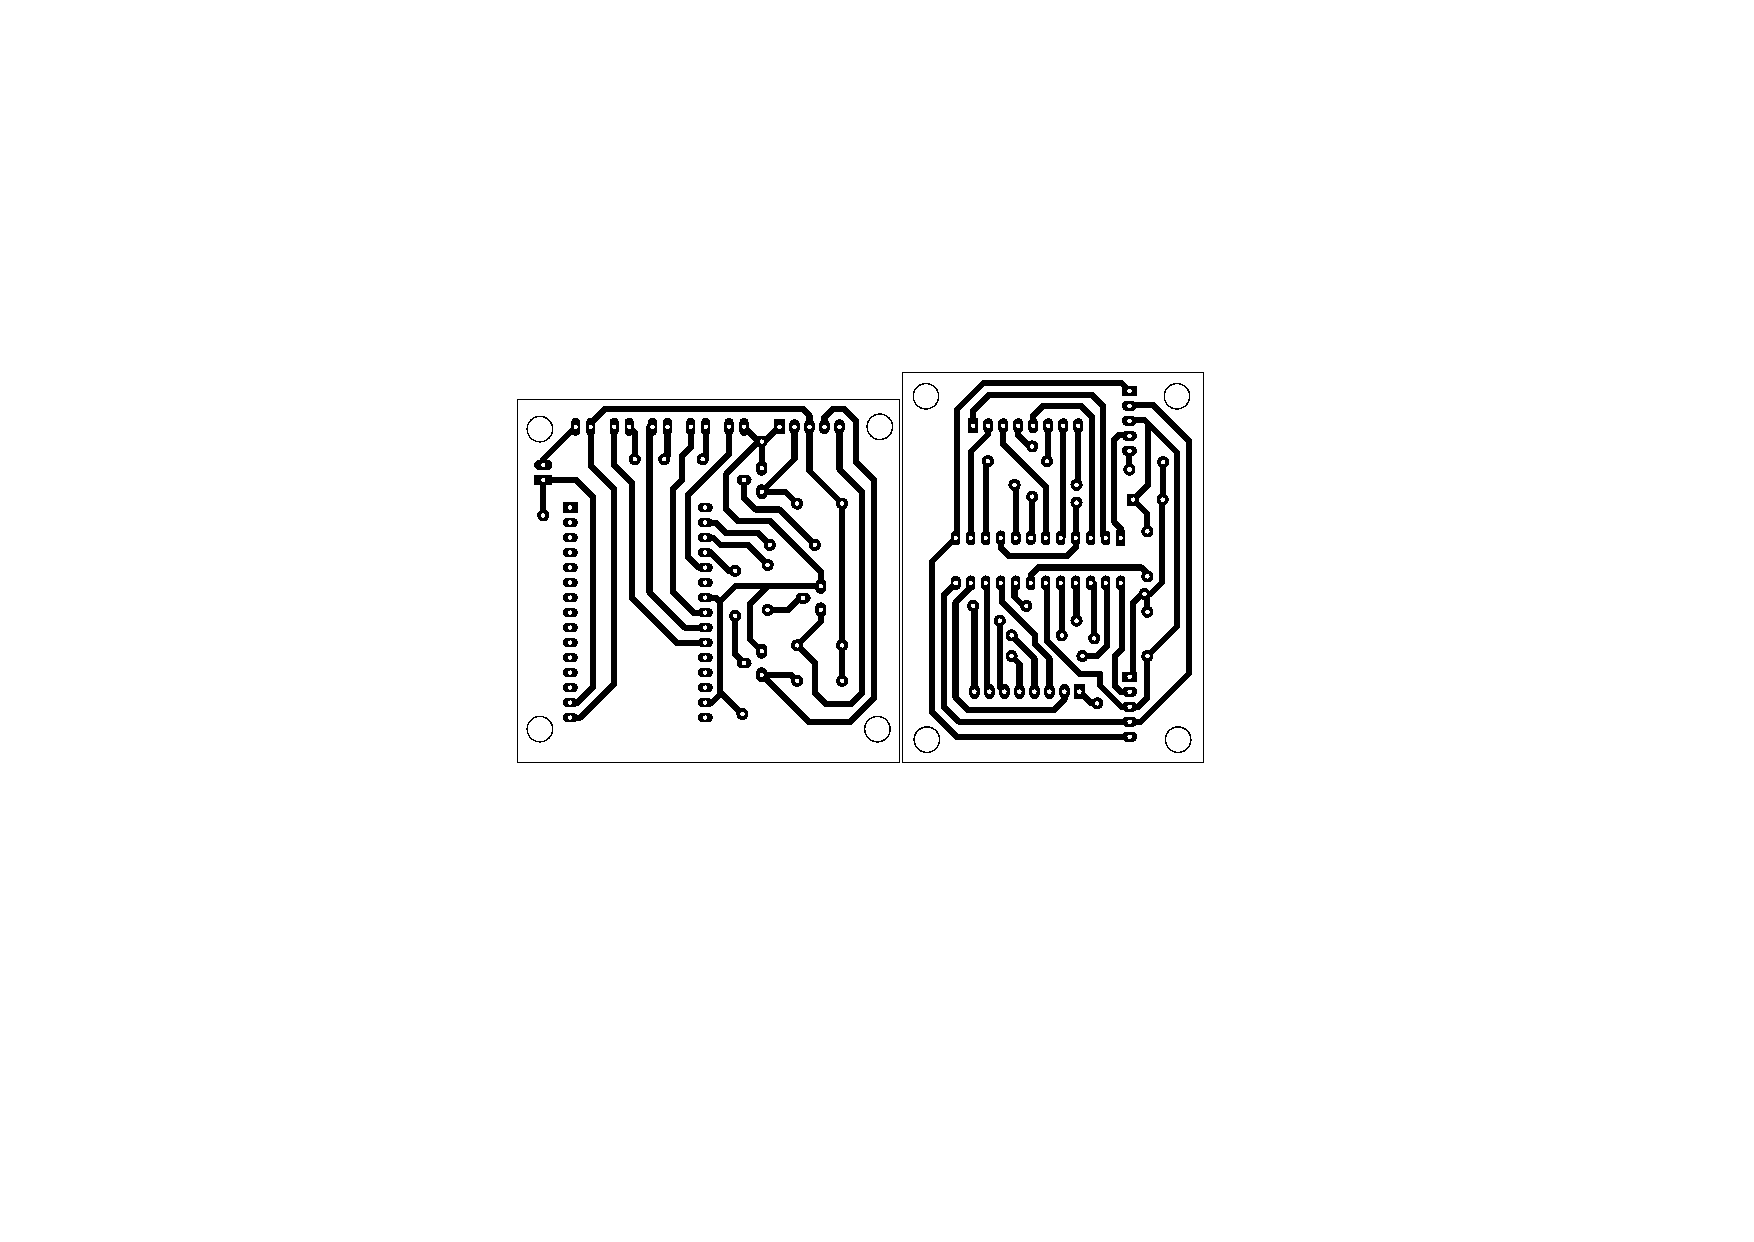
\includegraphics[width=\linewidth]{imagenes/hw/imp.pdf}
	\caption{Impresión PCB del módulo master y esclavo.}
	\label{fig:imp-pcb}
\end{figure}